\section{3D exploration strategies}

In contrast to 2D exploration and mapping strategies, mapping of large environments in 3D requires high memory and
computational consumptions. 
Different autonomous 3D exploration strategies were proposed so that 2D
exploration tools are used to three dimensions. In \cite{Joho2007}, Joho et al. presented an exploration strategy that extends the known 2D exploration strategies into the 3D space. Mapping is done using multi-level surface maps while a cost function takes
into account an expected information gain and a travel cost. 
Bachrach et
al. \cite{Bachrach2009} presented a solution for enabling a quadrotor helicopter to
autonomously explore and map unstructured indoor environments. Authors useed a 2D frontier-based exploration algorithm and set a fixed altitude for the helicopter
during exploration.  

Dornhege and Kleiner \cite{Dornhege2013} used a frontier based method extended to 3D exploration. This method requires high computational effort and operating environment is limited to small workspaces. On the other hand, Maurovic et al. \cite{Maurovic2014} presented a 3D exploration strategy for a mobile
robot equipped with a 3D laser scanner. This strategy ensures an on-line room detection algorithm focused on the room-by-room exploration keeping the memory and computational
requirements low.

Priyasad et al. \cite{Priyasad2018} presented a point cloud based algorithm which can be used in a situation where
the prior knowledge of the environment is highly inaccurate. The algorithm uses depth images to get a local map, which is expanded by searching for uncharted areas picking the next best
location to explore using a breadth first approach given a set of
constraints. The proposed algorithm exploits the maps in the 3D
space allowing the navigation system to perform effectively in uneven terrains. 

Next-best-view approach in the process of building 3D model of a real object used without any a priori information about the environment was described in \cite{VasquezGomez2014}. The algorithm determines each view to reconstruct an arbitrary object. Furthermore, authors proposed a method to deal with the uncertainty in sensor positioning.
Next-best-view approach for 3D exploration was presented by Bircher et. al. \cite{Bircher2016}. Authors presented a novel path planning algorithm for the autonomous exploration of an unknown area. The proposed planner finds the best branch in an on-line computed tree. The quality of the branch is determined by the amount of unmapped space that can be explored. The planner is capable of running online, onboard a robot with limited resources.

Baiming et al. \cite{Baiming2018} presented a new target points based trajectory planning algorithm to explore unknown space. The proposed method progressively plans long-term target point, intermediate target point, local target points,
and local trajectory within real time constraint. By tracking the trajectory, robot can efficiently explore the unknown space while avoiding obstacles.

Zhu et al. \cite{Zhu2015} developed a vision-based tool that performs autonomous exploration using an MAV equipped with 3D sensors. A real time frontier based exploration strategy is used to build maps that are stored in the OctoMap format (Fig. \ref{fig:octomap}).

\begin{figure}[t!]
	\centering
	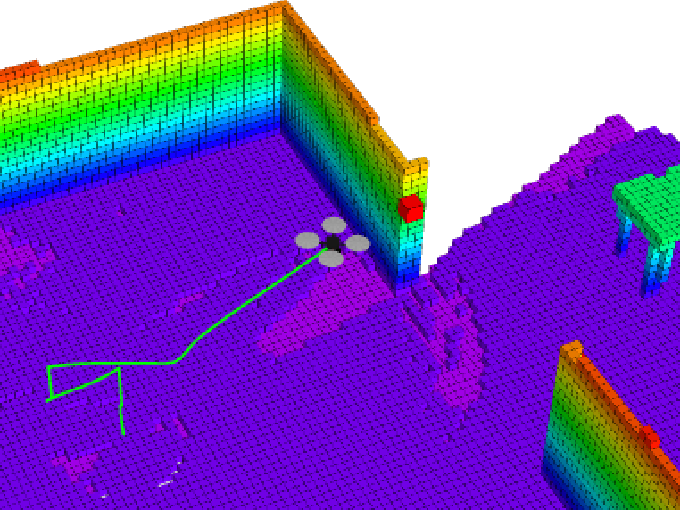
\includegraphics[width=1.0\columnwidth]{./pictures/octomap_and_drone.png}	
	\caption{UAV exploration in 3D environment. The colored voxels are 3D OctoMap representation and the green lines show the exploration trajectory \cite{Wang2019}.}
	\label{fig:octomap}
\end{figure}

Continuous cells are gathered into clusters and representative cells are chosen for each cluster. An evaluation function is used to choose the best representative cell and only state-changed space in the 3D map is processed in each iteration.
Authors in \cite{Senarathne2016} presened an alternative approach to 3D
exploration based on surface frontier voxels. The strategy focuses on seeking the expansion of mapped surfaces, instead of reducing unmapped voxels. 

Vutetakis in \cite{Vutetakis2019} proposed a novel startegy for inspecting
critical infrastructure autonomously using Micro Aerial Vehicles (MAV). In order to facilitate autonomous inspection capabilities, this strategy address the problem of autonomous MAV exploration and coverage of an unknown structure to acquire the spatial information necessary for the development of a high-fidelity 3D model of the structure. Key to this problem is to not only cover the entire structure, but also to minimize accumulative data errors during the exploration through direct planning of loop closures. 

Rocha et al. \cite{Rocha2005} dealt with 3D mapping by multi robots using cubic cells for information storage. Authors presented a technique which is used for frontier-based exploration. At the beginning of the exploration an initial map is given to the robot, the robots updates old map by new set information which calculate by measurement and shares their useful information with other robots. The process is repeated until whole area is explored and mapped.

Wang et al. \cite{Wang2018} studied the problem of autonomous exploration in unknown indoor environments using mutual information to evaluate the information the robot would get at a certain location. Authors proposed a
sampling method that can get random sensing patches in free space. In order to to collect information with true values, each sensing patch is extended to informative locations. They combined it with Gaussian
Markov Random Fields (GMRF) to model the distribution of mutual information in environment.  Authors also proposed a utility function that can balance the path cost and the information gain the robot
would collect.

The 3D exploration problem using aerial vehicles within limited flight endurance was addressed by Wang et al. \cite{Wang2019}. Authors proposed an information potential field based method considering both the traveled cost and information-gain. The next-best-view point is chosen based on a multi-objective function which considers information of several candidate regions and the traveled path cost. The selected goal
attracts the robot while known obstacles form the repulsive
force repel the robot.



\begin{figure}[t!]
	\centering
	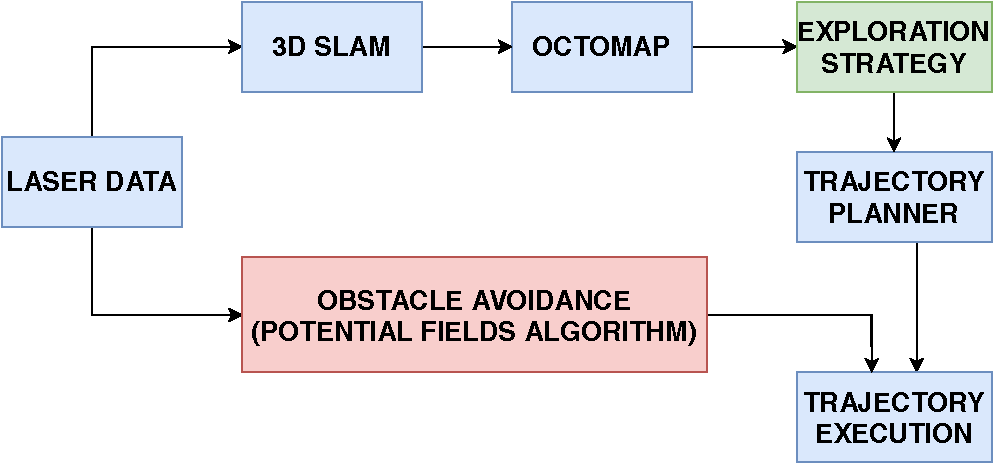
\includegraphics[width=1.0\columnwidth]{./pictures/3D_strategy.pdf}	
	\caption{Diagram of the implemented 3D exploration strategy.}
	\label{fig:3D_strategy}
\end{figure}


There are many algorithms to implement autonomous exploration as we described in the text above. Most of the algorithms are dependent on prior knowledge of the environment and apriori maps. Although
they are effective in some scenarios, these algorithms fail to
perform when the environment has been subjected to changes
that might invalidate the prior map. There are also algorithms implemented to deal with single robot exploration and mapping. Motivated by mentioned facts, we studied the problem of autonomous building exploration with purpose of fire detection. 
Besides
the localization and mapping of an unknown area, laser data is used for an OctoMap generation (Fig. \ref{fig:3D_strategy}). Google Cartographer SLAM crates a map in which a robot gets a goal point and using OctoMap generate trajectory and execute it. Obstacle avoidance is also considered in our work.